\chapter{Pilotage du projet et conception générale}

\section{Introduction}

Ce chapitre présente l'organisation du développement de la solution \textbf{AutoParts Pro} ainsi que les principaux choix effectués avant sa réalisation. Nous commençons par présenter le \textit{Product Backlog}, qui regroupe les fonctionnalités identifiées à partir des besoins de MSG, puis nous décrivons la répartition de ces fonctionnalités à travers les différents Sprints.

Nous présentons ensuite le diagramme de cas d'utilisation global afin de donner une vue d'ensemble des interactions entre les acteurs et la plateforme. La suite du chapitre est consacrée aux choix technologiques et aux outils utilisés durant le développement. Enfin, nous décrivons l'architecture générale de la solution et la répartition de ses différents composants.

%---------------------------------------------------------
\section{Pilotage du projet avec Scrum}

Afin d'organiser le développement de la plateforme \textbf{AutoParts Pro}, nous avons adopté une approche agile basée sur le cadre de travail Scrum. Ce choix permet de diviser le projet en plusieurs itérations et de développer progressivement les différentes fonctionnalités de la solution.

Le développement est ainsi organisé en plusieurs Sprints, chacun étant associé à un objectif fonctionnel précis. Cette organisation permet de suivre régulièrement l'avancement du projet, de tester les fonctionnalités développées et d'apporter des ajustements lorsque cela est nécessaire.

\subsection{Product Backlog}

Le \textit{Product Backlog} constitue une liste structurée des besoins fonctionnels identifiés pour la plateforme. Ces besoins sont exprimés sous forme de \textit{User Stories}, permettant de préciser l'acteur concerné, la fonctionnalité souhaitée et l'objectif recherché.

Les User Stories sont classées selon leur priorité et associées à une estimation de leur charge de réalisation. Le tableau~\ref{tab:product_backlog} présente une synthèse du backlog retenu pour notre projet.

\begin{table}[H]
    \centering
    \small
    \begin{tabular}{|c|p{3.4cm}|p{7.2cm}|c|c|}
        \hline
        \textbf{ID} &
        \textbf{Module} &
        \textbf{User Story} &
        \textbf{Priorité} &
        \textbf{Est.} \\
        \hline

        US1 &
        Authentification &
        En tant qu'utilisateur, je souhaite créer un compte et m'authentifier afin d'accéder aux fonctionnalités qui me sont autorisées. &
        Élevée &
        5j \\
        \hline

        US2 &
        Autorisations &
        En tant qu'Admin, je souhaite gérer les rôles et les permissions afin de contrôler l'accès aux différentes fonctionnalités. &
        Élevée &
        5j \\
        \hline

        US3 &
        Gestion des employés &
        En tant qu'Admin, je souhaite créer et gérer les comptes des employés ainsi que leurs départements. &
        Élevée &
        6j \\
        \hline

        US4 &
        Produits &
        En tant qu'Employee, je souhaite gérer les produits, catégories, marques et informations associées. &
        Élevée &
        7j \\
        \hline

        US5 &
        Stock &
        En tant qu'Employee, je souhaite consulter et gérer les stocks afin de suivre les mouvements des produits. &
        Élevée &
        7j \\
        \hline

        US6 &
        Fournisseurs &
        En tant qu'Employee, je souhaite gérer les fournisseurs et les opérations d'approvisionnement. &
        Moyenne &
        5j \\
        \hline

        US7 &
        E-commerce &
        En tant que Customer, je souhaite consulter et rechercher les pièces automobiles disponibles afin de trouver les produits adaptés à mes besoins. &
        Élevée &
        7j \\
        \hline

        US8 &
        Commandes &
        En tant que Customer, je souhaite gérer mon panier et passer une commande afin d'acheter les produits sélectionnés. &
        Élevée &
        7j \\
        \hline

        US9 &
        Paiements &
        En tant que Customer, je souhaite effectuer le paiement de ma commande et consulter les informations relatives à celui-ci. &
        Élevée &
        5j \\
        \hline

        US10 &
        Maintenance &
        En tant que Customer, je souhaite réserver un service de maintenance en renseignant les informations relatives à mon véhicule. &
        Élevée &
        8j \\
        \hline

        US11 &
        Interventions &
        En tant qu'Employee, je souhaite gérer les demandes de maintenance et suivre les interventions réalisées. &
        Élevée &
        7j \\
        \hline

        US12 &
        Ressources humaines &
        En tant qu'Admin, je souhaite gérer les informations des employés, les congés, les horaires et les shifts. &
        Moyenne &
        8j \\
        \hline

        US13 &
        Automatisation &
        En tant qu'administrateur, je souhaite automatiser certaines opérations afin de réduire les tâches répétitives. &
        Moyenne &
        6j \\
        \hline

    \end{tabular}
    \caption{Product Backlog du projet AutoParts Pro}
    \label{tab:product_backlog}
\end{table}

\subsection{Planification des Sprints}

Après l'identification des fonctionnalités, le Product Backlog a été réparti sur plusieurs Sprints en tenant compte des dépendances entre les modules et de leur priorité.

Le développement commence par les fonctionnalités nécessaires à la sécurisation de la plateforme. Les modules de gestion des produits et des stocks sont ensuite développés avant d'intégrer les fonctionnalités liées à la maintenance, aux ressources humaines et à l'automatisation.

Le tableau~\ref{tab:planification_sprints} présente la planification générale retenue.

\begin{table}[H]
    \centering
    \small
    \begin{tabular}{|c|p{4.2cm}|p{6.5cm}|c|}
        \hline
        \textbf{Sprint} &
        \textbf{Intitulé} &
        \textbf{Fonctionnalités principales} &
        \textbf{Période} \\
        \hline

        Sprint 0 &
        Initialisation du projet &
        Analyse des besoins, prise en main de l'environnement technique, définition de l'architecture et préparation du projet. &
        À préciser \\
        \hline

        Sprint 1 &
        Authentification et autorisations &
        Authentification, inscription, vérification e-mail, réinitialisation du mot de passe, JWT, rôles et permissions. &
        À préciser \\
        \hline

        Sprint 2 &
        Produits et gestion du stock &
        Gestion des produits, catégories, marques, fournisseurs et suivi des stocks. &
        À préciser \\
        \hline

        Sprint 3 &
        ERP et services de maintenance &
        Gestion des opérations ERP, réservations de maintenance, véhicules, demandes et interventions. &
        À préciser \\
        \hline

        Sprint 4 &
        Ressources humaines &
        Gestion des employés, départements, horaires, shifts et congés. &
        À préciser \\
        \hline

        Sprint 5 &
        E-commerce et automatisation &
        Commandes, paiements, factures, fonctionnalités e-commerce et automatisation des processus. &
        À préciser \\
        \hline

    \end{tabular}
    \caption{Planification des Sprints}
    \label{tab:planification_sprints}
\end{table}

Cette organisation permet de construire progressivement la solution en commençant par les fonctionnalités fondamentales, puis en ajoutant les différents modules métier. Les détails de chaque Sprint seront présentés dans les chapitres dédiés à leur réalisation.

%---------------------------------------------------------
\section{Diagramme de cas d'utilisation global}

Le diagramme de cas d'utilisation global permet de présenter les principales fonctionnalités de la plateforme ainsi que les interactions entre les différents acteurs.

Dans notre solution, trois utilisateurs principaux interagissent directement avec la plateforme : le \textbf{Customer}, l'\textbf{Employee} et l'\textbf{Admin}. Le système intervient également pour réaliser automatiquement certaines opérations, notamment l'envoi des e-mails et la gestion des mécanismes d'authentification.

Le \textbf{Customer} utilise principalement la partie e-commerce et les services de maintenance. Il peut créer son compte, consulter les produits, rechercher des pièces, gérer son panier, effectuer des commandes et réserver des interventions.

L'\textbf{Employee} intervient principalement dans la gestion opérationnelle de l'entreprise. Selon ses permissions, il peut gérer les produits, les stocks, les fournisseurs, les commandes ou encore les interventions de maintenance.

L'\textbf{Admin} dispose de fonctionnalités d'administration permettant notamment de gérer les employés, les départements, les rôles et les permissions.

Le diagramme permet ainsi d'avoir une vision globale du système avant d'étudier séparément les fonctionnalités de chaque Sprint.

%---------------------------------------------------------
% Figure du cas d'utilisation global
% Décommenter lorsque le diagramme sera disponible
%
%\begin{figure}[H]
%    \centering
%    \includegraphics[width=\textwidth]{images/uml/use_case_global.png}
%    \caption{Diagramme de cas d'utilisation global d'AutoParts Pro}
%    \label{fig:use_case_global}
%\end{figure}
%---------------------------------------------------------

\section{Choix techniques}

La réalisation d'AutoParts Pro nécessite plusieurs technologies permettant de couvrir les différents niveaux de la solution. Les choix techniques ont été effectués en tenant compte des besoins du projet, de la maintenabilité du code, de la sécurité et de la possibilité de faire évoluer la plateforme.

L'environnement technique est organisé autour de plusieurs éléments : le frontend destiné aux utilisateurs, le backend chargé de la logique métier, le système de gestion de données ainsi que les outils utilisés pour le développement et la collaboration.

\subsection{Environnement logiciel}

\subsubsection{Technologies du frontend}

\textbf{Angular} : est un framework open source développé par Google pour la conception d'applications web dynamiques. Il repose notamment sur TypeScript et propose une architecture basée sur les composants et les services.

Dans notre projet, Angular est utilisé pour développer les interfaces de l'application, notamment les interfaces d'administration de l'ERP et les différentes fonctionnalités accessibles aux utilisateurs.

\textbf{TypeScript} : est un langage développé par Microsoft qui étend JavaScript en ajoutant notamment le typage statique. Il facilite la structuration et la maintenance des applications web de grande taille.

TypeScript est utilisé dans notre projet pour développer les composants, services, modèles et différents éléments de l'application Angular.

\textbf{HTML5 et CSS3} : sont utilisés pour structurer et mettre en forme les interfaces web. Ils permettent de construire des interfaces adaptées aux différentes fonctionnalités de la plateforme.

\textbf{Tailwind CSS} : est utilisé pour faciliter la conception des interfaces et permettre une mise en page cohérente et adaptable aux différentes tailles d'écran.

\subsubsection{Technologies du backend}

\textbf{Java} : constitue le langage principal utilisé pour le développement de la partie serveur. Sa robustesse, son typage et son large écosystème en font une technologie adaptée à la réalisation d'applications métier.

\textbf{Spring Boot} : est un framework Java permettant de développer des applications backend de manière structurée et efficace. Il facilite notamment la création d'API REST et l'organisation de la logique métier.

Dans AutoParts Pro, Spring Boot assure le traitement des requêtes provenant du frontend, l'application des règles métier et l'accès aux données.

\textbf{Spring Security} : est utilisé pour mettre en place les mécanismes d'authentification et d'autorisation. Il permet notamment de sécuriser les ressources de l'application et de contrôler les accès selon les rôles et permissions.

\textbf{JWT} (\textit{JSON Web Token}) : est utilisé pour transmettre de manière sécurisée les informations nécessaires à l'authentification entre le frontend et le backend. Après une authentification réussie, un token est généré puis utilisé lors de l'accès aux ressources protégées.

\subsubsection{Système de gestion des données}

\textbf{MySQL} : est un système de gestion de bases de données relationnelles. Il permet de stocker et d'organiser les informations nécessaires au fonctionnement de la plateforme.

Dans notre projet, la base de données contient notamment les informations relatives aux utilisateurs, employés, produits, catégories, fournisseurs, stocks, commandes, paiements, factures et opérations de maintenance.

\textbf{Spring Data JPA} : est utilisé pour faciliter l'interaction entre l'application Java et la base de données. Il permet de manipuler les données à travers des repositories et de réduire le code nécessaire aux opérations courantes d'accès aux données.

%---------------------------------------------------------
\section{Outils de développement}

Plusieurs outils ont été utilisés afin de faciliter la réalisation, le test et la maintenance de la plateforme.

\subsection{Environnement de développement}

\textbf{Visual Studio Code} : est un éditeur de code utilisé principalement pour le développement de la partie Angular. Il propose de nombreuses extensions facilitant le développement TypeScript, Angular, HTML et CSS.

\textbf{IntelliJ IDEA} : est un environnement de développement intégré utilisé pour la réalisation de la partie backend Java et Spring Boot. Il fournit notamment des outils d'analyse du code, de débogage et de gestion des projets Maven.

\subsection{Outil de construction}

\textbf{Maven} : est utilisé pour gérer la construction du projet backend ainsi que les dépendances nécessaires à l'application Spring Boot. Il permet également d'automatiser différentes opérations liées au cycle de développement.

\subsection{Outils de gestion de versions}

\textbf{Git} : est un système de gestion de versions distribué permettant de conserver l'historique des modifications apportées au code source et de travailler avec différentes branches.

\textbf{GitHub} : est utilisé comme plateforme d'hébergement des dépôts Git. Il facilite la sauvegarde du code, la gestion des branches et le suivi des différentes versions du projet.

\subsection{Outil de gestion du projet}

\textbf{Trello} : peut être utilisé pour organiser les tâches du projet sous forme de tableaux et de cartes. Il permet de suivre l'état d'avancement des différentes User Stories et tâches associées aux Sprints.

%---------------------------------------------------------
\section{Outils de conception et de modélisation}

\textbf{PlantUML} : est un outil permettant de générer différents types de diagrammes à partir d'une description textuelle. Il est utilisé dans notre projet pour représenter notamment les diagrammes UML.

Cette approche facilite la modification des diagrammes au cours de l'évolution du projet et permet de conserver une représentation cohérente avec la conception du système.

Les diagrammes utilisés dans le cadre du projet comprennent principalement :

\begin{itemize}
    \item les diagrammes de cas d'utilisation ;
    \item les diagrammes de classes ;
    \item les diagrammes de séquence.
\end{itemize}

%---------------------------------------------------------
\section{Architecture de l'application}

Le choix de l'architecture représente une étape importante dans la conception d'AutoParts Pro. Une organisation claire des différentes responsabilités permet de faciliter la maintenance, l'évolution et la sécurisation de la plateforme.

Nous avons adopté une architecture en couches séparant principalement la présentation, la logique métier et l'accès aux données. Cette organisation permet de limiter les dépendances directes entre les différentes parties du système.

%---------------------------------------------------------
% Figure architecture
% Décommenter lorsque le diagramme sera disponible
%
%\begin{figure}[H]
%    \centering
%    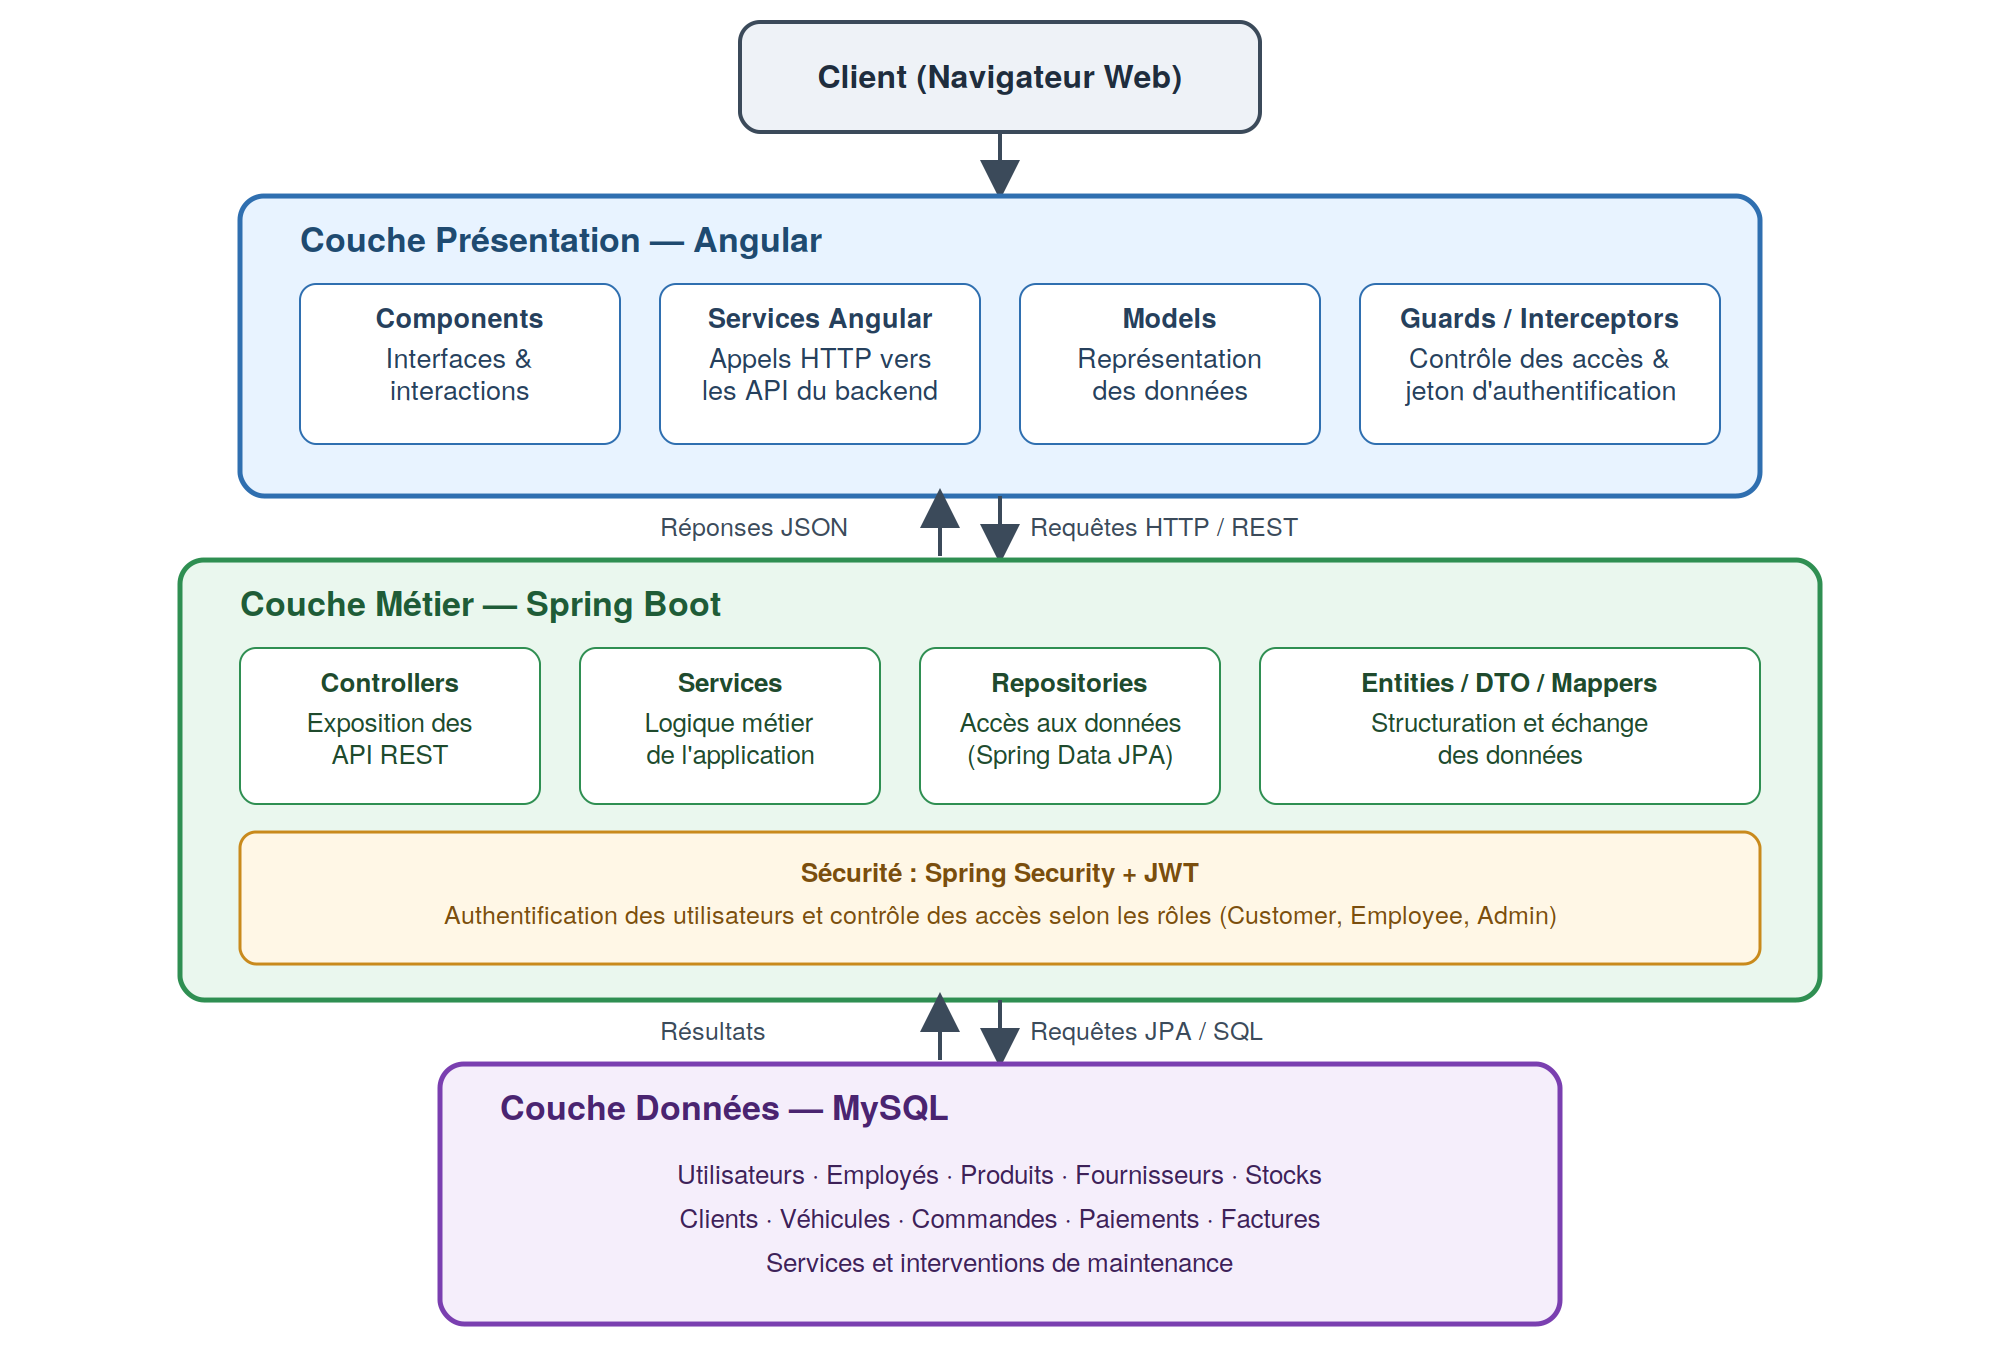
\includegraphics[width=\textwidth]{images/architecture/architecture_generale.png}
%    \caption{Architecture générale de la plateforme AutoParts Pro}
%    \label{fig:architecture_generale}
%\end{figure}
%---------------------------------------------------------

\subsection{Couche présentation}

La couche présentation correspond à l'application frontend développée avec Angular. Elle assure l'interaction avec les utilisateurs et prend en charge l'affichage des informations ainsi que la récupération des données depuis le backend.

Elle est principalement composée des éléments suivants :

\begin{itemize}

    \item \textbf{Components :}
    ils représentent les différentes interfaces et assurent la gestion des interactions avec les utilisateurs.

    \item \textbf{Services Angular :}
    ils assurent la communication avec le backend à travers des requêtes HTTP et permettent de centraliser les appels aux différentes API.

    \item \textbf{Models :}
    ils permettent de représenter côté frontend les données manipulées par l'application.

    \item \textbf{Guards et Interceptors :}
    ils participent à la sécurisation de l'application frontend, notamment en contrôlant l'accès aux routes et en ajoutant les informations d'authentification aux requêtes.
    
\end{itemize}

\subsection{Couche métier}

La couche métier correspond à l'application backend développée avec Spring Boot. Elle reçoit les requêtes provenant du frontend, applique les règles métier et retourne les résultats nécessaires.

Elle est organisée autour de plusieurs composants :

\begin{itemize}

    \item \textbf{Controllers :}
    ils reçoivent les requêtes HTTP et exposent les différentes API REST de l'application.

    \item \textbf{Services :}
    ils contiennent la logique métier et assurent le traitement des opérations demandées.

    \item \textbf{Repositories :}
    ils assurent l'accès aux données stockées dans la base de données.

    \item \textbf{Entities :}
    elles représentent les principales données métier manipulées par l'application et sont associées aux tables de la base de données.

    \item \textbf{DTO :}
    les objets de transfert de données permettent d'échanger uniquement les informations nécessaires entre le frontend et le backend.

    \item \textbf{Mappers :}
    ils assurent la conversion entre les entités métier et les DTO utilisés pour les échanges avec le frontend.

\end{itemize}

\subsection{Couche données}

La couche données correspond à la base de données relationnelle MySQL. Elle assure la persistance des informations utilisées par les différents modules de la plateforme.

Les données stockées concernent notamment :

\begin{itemize}
    \item les utilisateurs et leurs rôles ;
    \item les employés et les départements ;
    \item les produits, catégories et marques ;
    \item les fournisseurs et les stocks ;
    \item les clients et les véhicules ;
    \item les commandes et les lignes de commande ;
    \item les paiements et les factures ;
    \item les services et les interventions de maintenance.
\end{itemize}

Cette séparation en différentes couches permet de mieux organiser le code et de faciliter les évolutions futures de la plateforme.

%---------------------------------------------------------
\section{Architecture générale des échanges}

Le fonctionnement général de la plateforme repose sur une communication entre le frontend Angular et le backend Spring Boot à travers des API REST.

Lorsqu'un utilisateur effectue une opération depuis l'interface, le composant Angular concerné transmet la demande au service correspondant. Celui-ci envoie une requête HTTP vers l'API REST du backend.

Le contrôleur Spring Boot reçoit ensuite la requête et la transmet au service métier approprié. Le service applique les règles nécessaires et utilise les repositories pour accéder aux données stockées dans MySQL.

Une fois le traitement terminé, le résultat est retourné au frontend sous forme de données JSON afin d'être affiché à l'utilisateur.

Cette organisation permet de séparer clairement l'interface utilisateur, la logique métier et la persistance des données, tout en facilitant la maintenance et l'évolution de la solution.

%---------------------------------------------------------
\section{Conclusion}

Dans ce chapitre, nous avons présenté l'organisation du projet AutoParts Pro à travers le Product Backlog et la planification des différents Sprints. Nous avons également décrit le diagramme de cas d'utilisation global afin de présenter les principales interactions entre les acteurs et le système.

Nous avons ensuite présenté les technologies et les outils retenus pour le développement, notamment Angular, TypeScript, Java, Spring Boot, Spring Security, JWT et MySQL, ainsi que les outils utilisés pour le développement, la gestion des versions et la modélisation.

Enfin, l'architecture générale de la plateforme a été décrite en présentant les responsabilités des différentes couches et les échanges entre le frontend, le backend et la base de données.

Ces choix constituent la base technique et organisationnelle nécessaire à la réalisation progressive de la solution. Les chapitres suivants seront consacrés à la réalisation des différents Sprints et à la présentation détaillée des fonctionnalités développées.